\section{Simulative Evaluation of Hierarchical Caching Systems}\label{sec:hierarchical:simulative:simulative}

To evaluate the performance of a CDN supported by home routers, two scenarios are simulated. The first scenario simulates requests to a CDN with caches organized in a tree structure and compares isolated caches to cooperating caches to assess the benefit of the overlay.
The second scenario adds an AS topology with peering and transit links to evaluate the inter-domain traffic saving potential. As described in \refchap{chap:aslevel} a transit link exists between a customer ISP and its transit provider, if the customer ISP pays the transit provider to forward its traffic destined to parts of the Internet that the customer ISP does not own or cannot reach.

%\subsection{Caching}

To assess the impact of the number of shared home routers and the size of the ISP, a tiered caching architecture with resource locations at three different tiers, including the main data center of the content provider, CDN caches, and end-user equipment is evaluated.
%Table 6 3 shows the default parameters of the content delivery simulation.
The number of different content items to be downloaded or streamed from the resources is specified by the catalog size $N$. Tier-3 resource is the data center of the content provider, where all $N$ content items are stored. Tier-2 resources are edge caches and ISP caches, typically organized in a CDN, which are located close to Internet exchange points or within ISP networks. Requests served by ISPs or edge caches produce less or no inter-domain costs. Thus, these caches are referred as ISP caches in the following. The capacity of ISP caches is given as a fraction of $N$ and is specified by $C_{ISP}$. The caching strategy of ISP caches is LRU.
%Each autonomous system hosts an ISP cache.
Within tier-1, the caches are placed on shared home routers. These caches are referred to in the following as home routers (HRs). The cache capacity of HRs is specified by $C_{HR}$ and their caching strategy is LRU. In this study $C_{HR}$ is set to four (4) content items.

We evaluate the performance dependent on the autonomous system size $n_{user}$, in terms of the number of end-users in the autonomous system. The probability that an end-user enables the HR to shares contents is given by $p_{share}$. The probability that a user requests certain content items depends on the content's popularity distribution, which is specified by the Zipf exponent $\alpha$.

\subsection{Simulation Model}\label{sec:simeval}

The parameters considered in the content delivery simulation framework are
\begin{itemize}
  \item the resource distribution,
  \item the caching and content placement strategy,
  \item the resource selection strategy,
  \item the content demand,
  \item the AS-Topology.
\end{itemize}
Other considered parameters that are not relevant for this monograph, are
\begin{itemize}
  \item the social network of users,
  \item the video bitrate and chunk-size distribution,
  \item and the application and QoE.
\end{itemize}
In the following we briefly describe each of the parameter sets and provide models.

\subsubsection{Resource Distribution}
The resource distribution determines how video streaming sources are distributed among autonomous systems.
The number and size of autonomous systems is specified.
The size of an autonomous system is given by the number of end-users located in it.
In literature, the distribution of end-users on ASs is characterized as heterogeneous \cite{}.
We use a geometric distribution as a basic model for number of end-users in the ASs.
A more detailed model is developed using the Internet Census dataset, c.f. Section \refsec{}.
Video streaming sources can be a) data centers of the content provider, b) edge caches of the content provider, c) caches hosted by the ISP, d) home router / UNaDas, or e) end-user devices.
For each video streaming source the AS-location and its capacity is specified.
The capacity is given by the number of items that can be cached.
The size of the item catalogue is also specified in this parameter set.

TODO Bandwith constraints

\subsubsection{Caching and Content Placement Strategy}
The caching and content placement strategy determines in which video streaming source which video item is placed and when.
The content placement strategy is defined by the caching strategies of the individual caches.
In a distributed approach each cache decides based on the information it has which items to cache.
If global knowledge of the item demand is assumed, optimized content placement strategies such as hot warm cold.
Thus, the availability of items in ASs might for example be increased.
Each caching strategy is further defined by its specific parameters according to \refsec{}.

\subsubsection{Resource Selection Strategy}
The resource selection strategy determines from which cache instance an item is streamed when requested.
The simplest resource selection just selects a random resource.
By default, resources in tier-1 are selected first in hierarchical content delivery networks.
Other resource selection strategies that try to optimize different metrics were implemented, such as local resource selection, which tries to save inter-domain traffic by prioritizing caches in the order: home router / UNaDa in the same AS, ISP managed cache in the same AS, edge cache of content provider, data center of content provider.
%Further resource selection strategies that are not yet implemented could for example consider load balancing of the request based on the capacity of the caches.

\subsubsection{Social Network of Users}
The social network of users determines the friendship relationships between users. A basic model only defines the number of users in the system.
The number of friends of the user can be modeled by a power-law or geometric distribution.
A more detailed model specifies the friendship graph which consists of a node for each user and edges between users with friend relationships.
Friendship graphs have typical properties, such as a heavy-tailed in and out degree distribution.
In literature are different models for generating graphs with these properties.
A model used to generate social network graphs with varying size and density is the forest fire model \cite{}.
We further specify the feed size as parameter that represents the news feed of social network platforms.
The news feed is updated in sharing events.
Videos which are on the news feed of a user are watched with high probability.
Categories are defined by specifying the probability that a user is interested in a particular category.

\subsubsection{Traffic and Popularity Model}
The content demand determines the request rates of the video items.
Different demand models are implemented in the simulation, that reach from basic models that only consider the popularity distribution of the items to detailed models that consider temporal, spatial and social dynamics, c.f. \refsec{}.

The arrival process of video requests is specified by the inter-arrival time of video requests.
The request rate depends on the time of day and is generally lower at night.
The day is divided in short time slots, where the arrival rate does not change significantly, so that the arrival process can be assumed as quasi stationary.
In these time slots the arrival process is modeled as Poisson-process.
The parameter lambda of the arrival process depends on the popularity of the item and the time of day.
The probability of sharing a watched video is given by the sharing probability.

\subsubsection{AS Topology}
TODO AS Topology

Finally, Simulation parameters are specified that define the random number seed, the simulation time and the parameter study.

bandwidth constraints

transit costs

\subsubsection{Performance metrics}

To assess the performance of content delivery networks several metrics are considered:

\begin{itemize}
\item Cache hit rate:
\item Cache serve rate:
\item Cache contribution:
\item Inter-domain traffic:
\end{itemize}

\begin{figure}[bt]
  \centering
  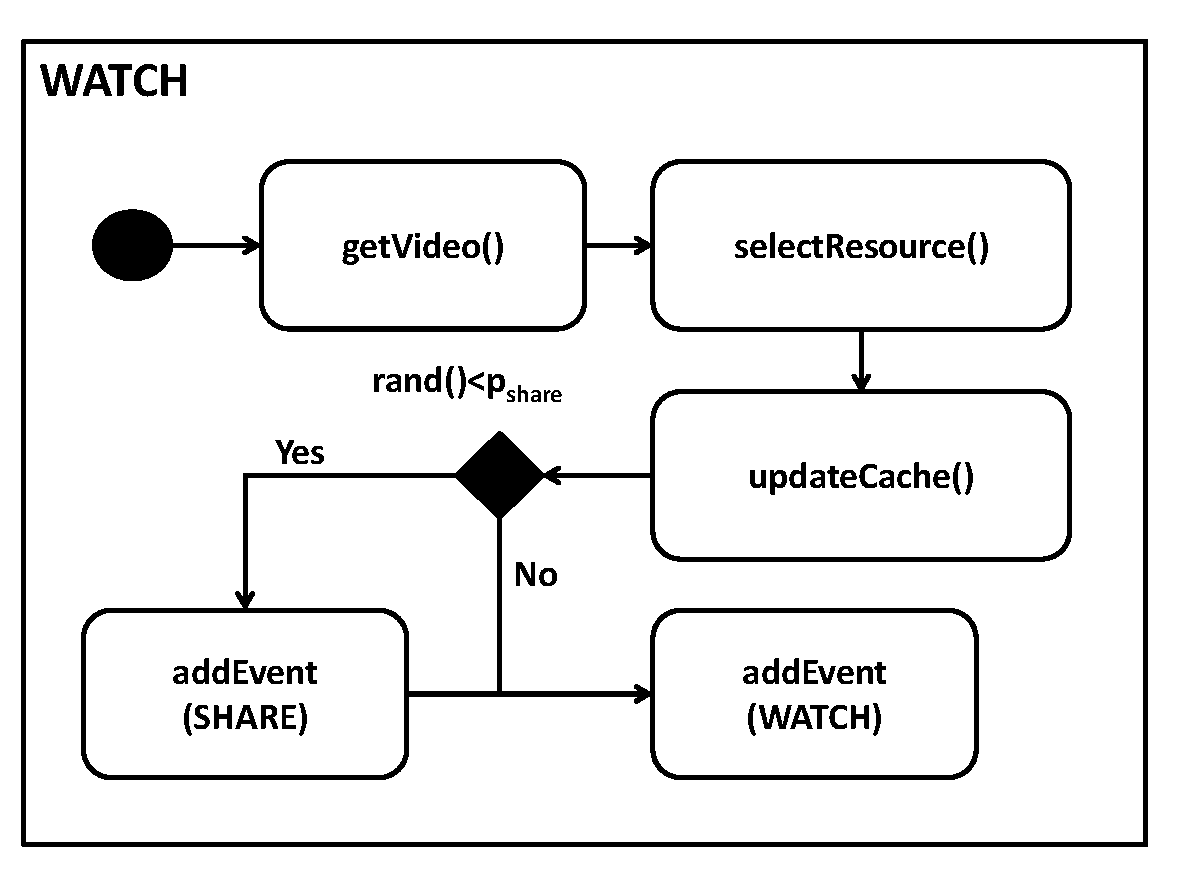
\includegraphics[width=0.6\textwidth]{hierarchical/simulative/figures/watch}
  \caption{Proccess diagram of a WATCH event.}
  \label{fig:WATCH}
\end{figure}

The content delivery simulation framework is implemented in MatLab.
The simulation is event-based including two major events.
First there is the WATCH event, which is processed when a user watches or consumes a video item.
Second there is a SHARE event, which simulates a sharing action of a user, where the video is posted on the news feeds in the social network.
\reffig{fig:WATCH} shows the process diagram of a WATCH event.
The process of a WATCH event starts by selecting a video dependent on the demand model specified in the parameters.
A video with video identifier $v_\text{id}$ is returned.
In the next step a cache or data center is selected that holds the item with $v_\text{id}$.
The download of the item from this resource is recorded in the statistics.
The cache identifier $c_\text{id}$ is returned and the cached items are updated according to the caching strategy specified in the parameters.
The user then decides to share $v_\text{id}$ with probability $p_\text{share}$.
In this case a SHARE event is added.
Finally, the next WATCH event is added according to the traffic and popularity model.

A SHARE event puts a given $v_\text{id}$, or a random video according to the user's interest on top of the news feed of the user's friends.
The user's friends are determined by the social graph.
The simulation is initialized with a WATCH event for each user.

The simulation framework is open source and available on github\footnote{\url{https://github.com/pettitor/content_delivery}}.
